%%%%%%%%%%%%%%%%%%%%%%%%%%%%%%%%%%%%%%%%%%%%%%%%%%%%%%%%%%%%%%%%%%%%%%%%%%%%%%%%%%%%%%%%%%%%%%%%%%%%%%%%%%%%%%%%%%%%%%%%%%%%%%%%%%%%%%%%%%%%%%%%%%%%%%%%%%%
% This is just an example/guide for you to refer to when submitting manuscripts to Frontiers, it is not mandatory to use Frontiers .cls files nor frontiers.tex  %
% This will only generate the Manuscript, the final article will be typeset by Frontiers after acceptance.   
%                                              %
%                                                                                                                                                         %
% When submitting your files, remember to upload this *tex file, the pdf generated with it, the *bib file (if bibliography is not within the *tex) and all the figures.
%%%%%%%%%%%%%%%%%%%%%%%%%%%%%%%%%%%%%%%%%%%%%%%%%%%%%%%%%%%%%%%%%%%%%%%%%%%%%%%%%%%%%%%%%%%%%%%%%%%%%%%%%%%%%%%%%%%%%%%%%%%%%%%%%%%%%%%%%%%%%%%%%%%%%%%%%%%

%%% Version 3.3 Generated 2016/11/10 %%%
%%% You will need to have the following packages installed: datetime, fmtcount, etoolbox, fcprefix, which are normally inlcuded in WinEdt. %%%
%%% In http://www.ctan.org/ you can find the packages and how to install them, if necessary. %%%
%%%  NB logo1.jpg is required in the path in order to correctly compile front page header %%%

\documentclass[utf8]{frontiersSCNS} % for Science, Engineering and Humanities and Social Sciences articles
%\documentclass[utf8]{frontiersHLTH} % for Health articles
%\documentclass[utf8]{frontiersFPHY} % for Physics and Applied Mathematics and Statistics articles

%\setcitestyle{square} % for Physics and Applied Mathematics and Statistics articles
\usepackage{url,hyperref,lineno,microtype,subcaption}
\usepackage[onehalfspacing]{setspace}
\usepackage{graphicx}
\usepackage{listings}
\usepackage{color}
\usepackage{lscape}
\usepackage[T1]{fontenc}
\usepackage{tikz}
\usepackage[colorinlistoftodos]{todonotes}


\definecolor{mygreen}{rgb}{0,0.6,0}
\definecolor{mygray}{rgb}{0.5,0.5,0.5}
\definecolor{mymauve}{rgb}{0.58,0,0.82}

\lstset{ %
  backgroundcolor=\color{white},   % choose the background color; you must add \usepackage{color} or \usepackage{xcolor}; should come as last argument
  basicstyle=\footnotesize,        % the size of the fonts that are used for the code
  breakatwhitespace=false,         % sets if automatic breaks should only happen at whitespace
  breaklines=true,                 % sets automatic line breaking
  captionpos=b,                    % sets the caption-position to bottom
  commentstyle=\color{mygreen},    % comment style
  deletekeywords={...},            % if you want to delete keywords from the given language
  escapeinside={\%*}{*)},          % if you want to add LaTeX within your code
  extendedchars=true,              % lets you use non-ASCII characters; for 8-bits encodings only, does not work with UTF-8
  frame=single,	                   % adds a frame around the code
  keepspaces=true,                 % keeps spaces in text, useful for keeping indentation of code (possibly needs columns=flexible)
  keywordstyle=\color{blue},       % keyword style
  language=Octave,                 % the language of the code
  morekeywords={*,...},            % if you want to add more keywords to the set
  numbers=left,                    % where to put the line-numbers; possible values are (none, left, right)
  numbersep=5pt,                   % how far the line-numbers are from the code
  numberstyle=\tiny\color{mygray}, % the style that is used for the line-numbers
  rulecolor=\color{black},         % if not set, the frame-color may be changed on line-breaks within not-black text (e.g. comments (green here))
  showspaces=false,                % show spaces everywhere adding particular underscores; it overrides 'showstringspaces'
  showstringspaces=false,          % underline spaces within strings only
  showtabs=false,                  % show tabs within strings adding particular underscores
  stepnumber=2,                    % the step between two line-numbers. If it's 1, each line will be numbered
  stringstyle=\color{mymauve},     % string literal style
  tabsize=2,	                   % sets default tabsize to 2 spaces
  title=\lstname                   % show the filename of files included with \lstinputlisting; also try caption instead of title
}



% Leave a blank line between paragraphs instead of using \\


\def\keyFont{\fontsize{8}{11}\helveticabold }
\def\firstAuthorLast{Sample {et~al.}} %use et al only if is more than 1 author
\def\Authors{First Author\,$^{1,*}$, Co-Author\,$^{2}$ and Co-Author\,$^{1,2}$}
% Affiliations should be keyed to the author's name with superscript numbers and be listed as follows: Laboratory, Institute, Department, Organization, City, State abbreviation (USA, Canada, Australia), and Country (without detailed address information such as city zip codes or street names).
% If one of the authors has a change of address, list the new address below the correspondence details using a superscript symbol and use the same symbol to indicate the author in the author list.
\def\Address{$^{1}$Laboratory X, Institute X, Department X, Organization X, City X , State XX (only USA, Canada and Australia), Country X \\
$^{2}$Laboratory X, Institute X, Department X, Organization X, City X , State XX (only USA, Canada and Australia), Country X  }
% The Corresponding Author should be marked with an asterisk
% Provide the exact contact address (this time including street name and city zip code) and email of the corresponding author
\def\corrAuthor{Corresponding Author}

\def\corrEmail{email@uni.edu}




\begin{document}
\onecolumn
\firstpage{1}

\title[NWB Query Engine]{NWB Query Engine: Efficient way to query neurophysiological data stored in Neurodata Without Borders format} 

\author[\firstAuthorLast ]{\Authors} %This field will be automatically populated
\address{} %This field will be automatically populated
\correspondance{} %This field will be automatically populated

\extraAuth{}% If there are more than 1 corresponding author, comment this line and uncomment the next one.
%\extraAuth{corresponding Author2 \\ Laboratory X2, Institute X2, Department X2, Organization X2, Street X2, City X2 , State XX2 (only USA, Canada and Australia), Zip Code2, X2 Country X2, email2@uni2.edu}


\maketitle
  

\begin{abstract}

%%% Leave the Abstract empty if your article does not require one, please see the Summary Table for full details.
\section{}
For full guidelines regarding your manuscript please refer to \href{http://www.frontiersin.org/about/AuthorGuidelines}{Author Guidelines}.

As a primary goal, the abstract should render the general significance and conceptual advance of the work clearly accessible to a broad readership. References should not be cited in the abstract. Leave the Abstract empty if your article does not require one, please see \href{http://www.frontiersin.org/about/AuthorGuidelines#SummaryTable}{Summary Table} for details according to article type. 


\tiny
 \keyFont{ \section{Keywords:} keyword, keyword, keyword, keyword, keyword, keyword, keyword, keyword} %All article types: you may provide up to 8 keywords; at least 5 are mandatory.
\end{abstract}


\section{Introduction}
  

Data from neuroscience experiments are heterogeneous and stored in various data formats. A data format is usually given by hardware and software equipment defined by a device vendor. Such proprietary formats cannot be easily changed or reused. With increasing number of experiments the proliferation of non-standardized data formats makes the effective management and sharing of data difficult. Researchers point out that data are even more important then papers describing results observed from the data. If results are described in scientific papers without access to the original datasets their validation or refinement over time is practically impossible. With increasing computational performance and disks capacity researchers are more motivated to preserve not only experimental results but also original data used for analysis. In last decades several attempts to provide a standardized way of data storing have appeared.

Huge volumes of produced data advance techniques of artificial intelligence (AI) for obtaining relevant information from various data sources. Hypotheses gained by AI techniques from biomedical databases and scientific papers are less error prone than hypotheses gained by human \citep{Gil171}.

Neurophysiological data are multimodal and dynamic because a single experiment can involve several signal acquisition modalities. The neuroscience community that is required to adopt a culture of data sharing and open access except of technological barriers is also facing a lot of barriers sociological and ethical \citep{10.3389/fnhum.2014.00239}.

With increasing amount of data a concept of so-called Big Data, most often defined as three Vs\citep{mcafee2012big} penetrates to neuroscience as well.

The usage of a Big Data concept is studied in \citep{10.3389/fvets.2017.00194}. They explore the concept of Big Data as an approach towards to the concept of one medicine. This approach is focused on a development of analytics and predictive methods, and models that optimize the translation of huge volumes of biomedical data into clinical practice. These methods profit from the ability to integrate information from diverse sources. Individual sources are supposed small but collectively represents a huge amount of knowledge.

A commentary \citep{Ferguson2014} defines so-called long-tail data as small and granular datasets collected by individual laboratories. They say that a culture of routine data sharing practically does not exist or at least the amount of shared data is minimal relative to the total amount of data produced. They recommend usage of public repositories maintained by independent organizations rather then the usage of private laboratory web pages. Then long-tail data stored in public repositories can be accessed and analyzed by Big Data techniques.


A requirement for a database infrastructure and technology that enable more rapid and comprehensive pursuit of the brain's physiology and pathophysiology is described in \citep{Insel2004}. Three areas of need are defined: (1) Understanding  where and when genes and the proteins they encodes are expressed in the mammalian brain, (2) finding better ways to manage information in existing databases to maximize their utility, and (3) integrating of various clinical programs such as epidemiology, genetics and therapeutics.

Many of problems with lack of data standards is related to an absence of an adequately trained work force.  According to the iNeuro workshop \citep{10.3389/fninf.2016.00028} there is only very few institutions with programs focused on a big data in neuroscience. Participant of this workshop endorsed student-centered, hand-on, and solving real problems training.

Problems of open data ecosystem from the point of technical and practical challenges, problems of data diversity, and existing marketplace is described in \citep{WIENER2016617}. Future recommendations from the point of incentives, discoverability and sustainability are described.
 
Another solutions are based on data descriptions by Semantic Web technologies which aim to make machine readable data accessible via the Internet.  One example is NEMO \citep{DouFRFMT07} that describes classes of event-related brain potentials (ERP) and their properties. Another example is OBI \citep{citeulike:7291351}  that contains both general terms useful for any kind of experiment and also terms for specific experiments. Every term has a unique identifier, standard metadata, and logical definitions that connect it to other terms in OBI. OEN \citep{10.3389/conf.fninf.2014.18.00044} aims to cover devices and methods, and a neurophysiological concepts derived from various data sources. 

There are also approaches not based on the usage of the Semantic Web Technologies but implement a concept of controlled vocabularies. It includes e.g odML terminologies\footnote{http://portal.g-node.org/odml/terminologies/v1.0/terminologies.xml} implemented in odML data format \citep{10.3389/fninf.2011.00016}.

Data are typically queried by languages such as SQL for relational databases or SPARQL\citep{prudhommeaux2008sparql} for the semantic web. However there is a gap in providing an easy-to-use query engine that is not bounded with a specific technology relying on a relational database or a SPARQL endpoint. The initial idea of SQL was to provide a language semantically and syntactically close to a natural language. Data were supposed easily accessible by a unified way without having knowledge of relational databases design. However it did not happen. Although SQL is a powerful language providing sufficient means for querying stored data its complexity requires a certain level of database systems knowledge. The SPARQL language is based on a similar concept but focused on RDF triples instead of a relational schema. The complexity of SPARQL makes it difficult to use by a non semantic web experts also.

To bring data closer to users data stored in relational databases are usually accessed by application programs. These programs must provide mapping of data from databases to a user interface (e. g. DataJoint \citep{Yatsenko031658}). Such programs are responsible for creating SQL queries according to user inputs. Anyway it requires continuous effort in maintaining of programs by application programmers especially when a data model is changed. This effort is dependent on manpower that must be available all the time. 

To address issues with non existing data format for neurophysiology data, the Neurodata Without Borders Cellular Neurophysiology (NWB:CN or just NWB) format was developed \citep{teeters-neuron}. The NWB data format, implemented in HDF5 container, provides a standard way to store cellular neurophysiology data and metadata. It was originally based on rodent data, but is being expanded to new types of data. 

Once the first pilot version of the format and the API has been released questions on how to effectively query data stored in the NWB format arose. Because a satisfactory query engine for file-based data formats does not exist we have developed a NWB query engine that provides an approach allowing query data in NWB files. Although a main motivation of this paper is driven by a lack of a query engine for the NWB data format we bring a solution that is general to allow querying data in other formats also. It resulted in the development of a query language, simpler then SQL or SPARQL that is independent of an implementation of specific data storage.

A practical implementation of a data connector to the NWB data format validates presented approach. The usage for other formats can be done by implementing another connector.

The paper is organized as follows: Section \ref{materials_and_methods} describes state of the art in developing of data formats for neurophysiological experiments, existing frameworks for querying stored data, and defines use-cases and specifications of the query engine. Then Section  \ref{results}  deals with the developed architectonic concept, describes implementation details and a user guide. Last Section  \ref{Discussion} compares limitations of existing systems with the current one and it points a future work. 

\section{Material and Methods}
\label{materials_and_methods}


\subsection{DataJoint}
\label{DataJoint}

DataJoint \citep{Yatsenko031658} is a tool aims to hide a complexity of relational schema and provide to users a use-friendly Python or Matlab API for easy integration of the data storage with the clients system. Technically it can be understand as an object-relational mapping \citep{Keith2010} for Matlab or Python based systems. The implementation maps database tables to Python classes allowing fetching data stored in the database to the instances of classes. DataJoint also defines basic operations on tuples such as conjunction: \emph{A \& B} denoting relations comprising all tuples from A that match any tuple in B. Disjunction: \emph{A * B} denoting relations comprising tuples in A and in B. Inverse: \emph{A - B} denoting all tuples from A that do not match any tuple in B. Projection: \emph{A.pro(B)} that modifies heading of A by B.

\subsection{HDF5}
\label{HDF5}

The HDF5 format is interesting in neuroscience community because provide multidimensional data storage and retrieval and also provides a sufficient way for storing experimental metadata. Moreover HDF5 provides nearly unlimited flexibility of datatypes. Another HDF5 group or dataset, or another file can be accessed by system of hard, soft or external links respectively. The other HDF5 applications \citep{Folk:2011:OHT:1966895.1966900} provide a high-level interface, DBMS Back-End, OPeNDAP support etc.


HDF5 format \citep{Koziol2011} provides following primitives to represent data:

\begin{itemize}
 \item Group - It is an element for grouping datasets into logical group. Group can be understood as a directory on a file system. Each file contains at least one group called root group
 \item Dataset - Is a representation of stored raw data. It is implemented as a multidimensional array 
 \item Attribute - Attribute is a key-value information used to supplement a group or a dataset by metadata
\end{itemize}

One drawback is that it does not support searching of data.


As a solution several attempts to provide a searching capability over HDF5 files has been proposed. HDF5-FastQuery \citep{1644309}, \citep{6114446} provides an approach for indexing on multi-dimensional data. The proposed API simplifies the execution of queries on HDF5 files for general scientific applications and data analysis.

Another approach \citep{6546110} creates a light-weight data management layer that allows running queries expressed in the SQL syntax on the metadata storage. The metadata are generated from HDF5 files in runtime.

Last tested, HDFql\footnote{\url{http://www.hdfql.com/}} facilitates working with HDF5 files by providing a SQL-like language with CREATE, INSERT, SELECT or SHOW operations. Using these operations a user can easily create and read new datasets, groups or attributes. 


\subsection{Neurodata Without Borders Format}
\label{nwb}

The aim of the Neurodata Without Borders project is to design a data format for storing a variety of neurophysiology data, including intracellular and extracellular electrophysiology experiments, optical physiology experiments, as well as tracking and stimulus data.

From the implementation point of view the HDF5 data format is used. This format is suitable because its easy-to-use, it does not require any specific software equipment installed on a user computer. It can be easily transferred between different computers and its internal structure provides sufficient means for storing both raw signal data and their metadata. The easy usability motivates several neuroscience initiatives and groups to implement their solution in HDF5 format as well. The NIX\footnote{\url{https://github.com/G-Node/nix}} format defines a structure for storing raw data as a groups and datasets within one HDF5 file together with metadata defined in their odML \citep{10.3389/fninf.2011.00016} format. Next,  Klustakwik\footnote{\url{http://klusta.readthedocs.io/en/latest/}} its an implementation of a Kwik format for storage of spike sorting data. The Kwik format is implemented in HDF5 BRAINformat \citep{10.3389/fninf.2016.00048} is a general framework for management of scientific data formats by their own concept of Managed Object representing individual semantic components of data formats.   Orca\footnote{\url{http://crcns.org/files/data/nwb/h1/NWBh1\_09\_Keith\_Godfrey.pdf}} is a HDF5 format for storing electrophysiology and optophysiology data and practically it is a predecessor of the NWB format.

Version 1.0 of the NWB format is available. Vesion 2.0 is currently under development removes some drawback of the previous one and adds a high-level API definition. The NWB Query Engine is fully compatible and tested on the version 1.0. Moreover its internal implementation is designed to be compatible also with version 2.0. 

The NWB data format defines a format specification language describing a hierarchy of stored metadata. There are two types of Metadata: (i) Metadata that are a part of a core format, and (ii) metadata that are not defined by the core format, but which are defined by extensions written in the specification language. When an extension is used a result file contains a merge of the core format metadata and the extension metadata.


\subsubsection{Data Types}
\label{data-types}

The experiments produce data of neuronal activity and behavioral measures from animals and humans. They consists largely of time series of measurements at varying sampling rates and associated metadata describing task parameters, anatomical locations of electrodes, etc. Moreover, they are organized in sessions hierarchically by subject / animal with multiple days of data per animal.

\subsubsection{Typical Experimental Data and Metadata}
\label{typical-data-analysis-steps}

Typical experiment contains several steps that are needed to set up an environment and to arrange recordings. During recording data are collected by a measuring device. This device reads usually time series data from an amplifier. These data are stored on a measuring computer. When experiments ends stored data are supplemented by descriptive metadata to be ready for archiving. The following text lists the most often stored metadata from animal and human recording. The description is a high-level set of metadata typical for most experiments. For specific purposes a more accurate metadata with more specific granularity can appear.

Typical animal recording contains following metadata groups:

\begin{itemize}
 \item Epochs information - names with start and end times for each period is stored together with information such as exposure number. 
 \item Electrode location - anatomical location for each electrode
 \item Cell properties information - clustered cells information
 \item Local field from potentials from each electrode - Filtered in different ranges (LFP, Ripple, Theta, etc.)
 \item LFP Events - Start and end time
 \item Animal position
 \item Times of task events
\end{itemize}

For human recording following metadata are typically stored:

\begin{itemize}
 \item Epochs information - names with start and end times for each period is stored together with information such as exposure number
 \item Electrode location - anatomical location for each electrode in native and standard atlas space.
 \item Potentials from each electrode - including multiple different ranges (LFP, deltha, theta, alpha, gamma etc.)
 \item Start end stop time of specific detected event
 \item Signal artifacts - movement, bad electrode etc.
 \item Stimulus information - time of stimulus onset, stimulus name, stimulus type and stimulus metadata
\end{itemize}



\subsection{Query Engine High Level Specification}
\label{Query_engine_specification}

According to typical scenarios defined in Section \ref{typical-data-analysis-steps} and data types defined in Section \ref{data-types} a minimal set of requirements on a NWB query engine have been defined.

A specification of the NWB query engine should ensure at least following functionality:
\begin{enumerate}
 \item To provide a simple query language that can specifying particular subsets of data for analysis based on searches of metadata and specific sets of times defined by those metadata or by intermediate analyses.
 \item To provide a read API for the NWB format data files that can quickly and easily be used to load up a set of requested data types at times constrained by the user’s query.
 \item To allow for the construction of query pipelines.
\end{enumerate}


\subsection{Scope and Requirements}
\label{Scope_and_requirements}

Because HDF5 (Section \ref{HDF5}) is the container for the NWB format (Section \ref{nwb}), the query engine is supposed to run on the top of an HDF5 file. Moreover, the definition of data types (Section \ref{data-types}) gives an idea of what items are required for searching. Typical analysis steps (Section \ref{typical-data-analysis-steps}) define conditions and restrictions that are applied to searched metadata. Also basic logical, arithmetical and relational math operators have to be implemented to support conjunction, disjunction, or intersection of partial results. Moreover, solutions as DataJoint mapping data from common relational-databases to python language must be taken into account because lot of scientific data is stored in relational databases. The implementation should not be narrowly focused only on NWB format but it should provide an easy extension possibilities to other platforms. From the users perspective because lot of tools in neuroscience are implemented in Python a way for calling the query engine from a Python code must be ensured. Moreover the system must be also usable for users who are not primarily programmers and must be accessible from common laboratory computers without requiring to install special programming environment.

\section{Results}
\label{results}


\subsection{Architecture}
\label{Architecture}

Because requirements defined in Section \ref{Scope_and_requirements} a modular architecture is required. It requires to implement a query mechanism independent of a concrete way of storing data. The NWB query engine contains three main components. The first component is a Query parser that takes a user input and parses a query according to a grammar described later in Section \ref{Query_Grammar}. The query is then split out to a subqueries and a subexpressions tree is generated. Such expressions are managed by a next block: NWB Processor. The NWB Processor iterates over the list of expressions to perform the specified queries  in the NWB file accessed by a HDF5 Connector. The HDF5 connector is a part of third block; a File API. Data obtained from the NWB file are returned back to the NWB Processor where they are wrapped in a NWB result object.

The python server is a component that enables users to run the engine as a python server. This server runs on a local or a remote host and allows running of queries from python code.

In order to make working with the engine even simpler we also developed a Web interface allowing to run the engine in a web container. Then data stored on a host server are accessed from a simple web pages that enables running of queries in a google-like search box. When matching files are found the user can download them from the remote server to a local machine.

\begin{figure}
% Use the relevant command to insert your figure file.
% For example, with the graphicx package use
  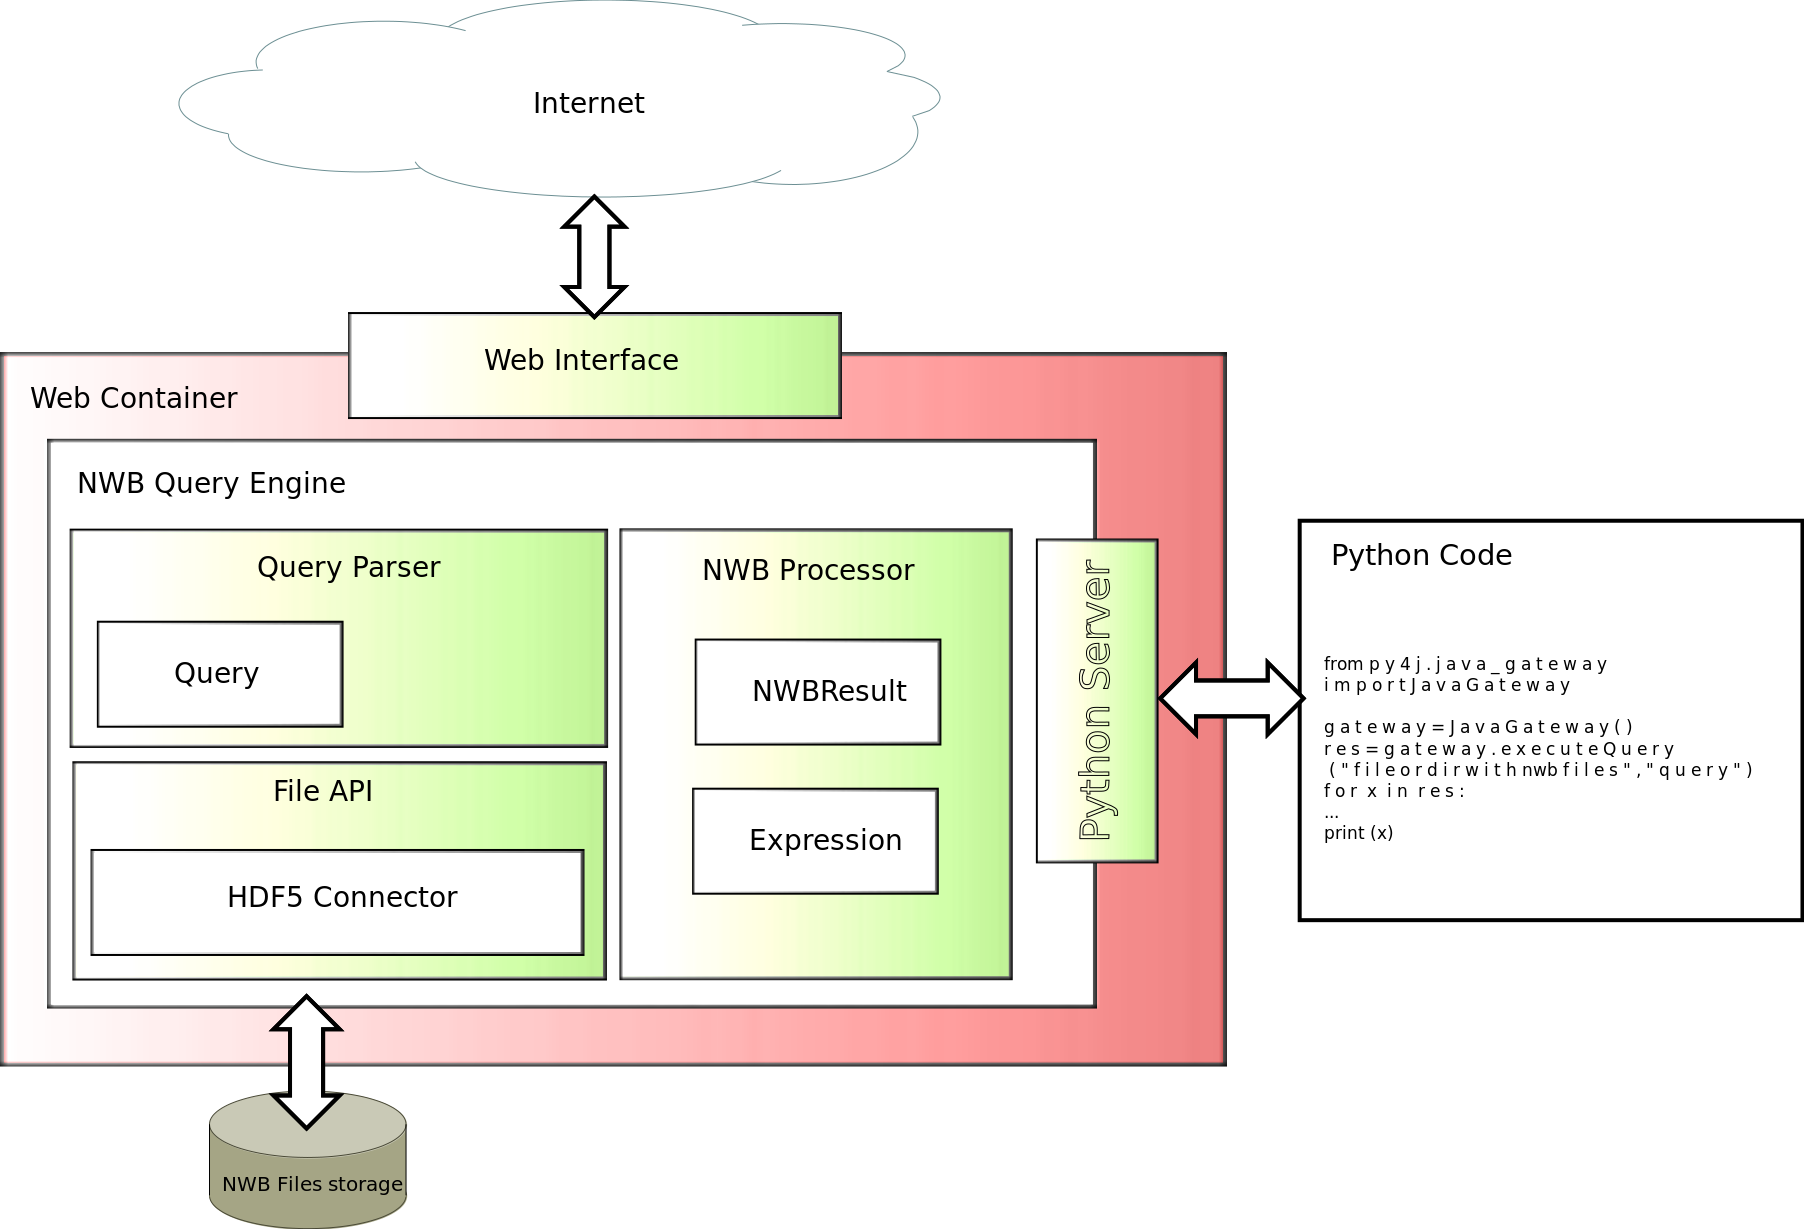
\includegraphics[width=17cm]{architecture}
% figure caption is below the figure
\caption{\textbf{Block Diagram of the Architecture of the NWB Query Engine. } A block NWB Query Engine is a core component including a Query Parser, File API and NWB Processor. The query parser translates a user input into an internal tree representation. The NWB Processor creates individual expressions from this tree. These expressions are executed in a NWB file by an HDF5 Connector. Then obtained data are wrapped in a NWBResult object that is returned back to the user. The individual blocks communicates via interfaces to facilitates its extension for different data storage. The Python server block enables running of the query engine as a python endpoint called from a python code. The block Web Interface. It represents an additional tool the NWB Query Engine Web Interface is a user-friendly web page allowing running of queries from a web browser.}
\label{fig:architecture}
\end{figure}


\subsection{Query Grammar}
\label{Query_Grammar}

Each query contains two parts separated by an "=". The left side is the name of target group or a dataset. The right side contains the name of a child of the target (i.e. an attribute or a dataset) together with a value restriction. Following operators are supported to define the value restrictions and logical operators allowing relational operations:

\begin{itemize}
 \item and \&
 \item or  |
 \item equal ==
 \item assignment =
 \item brackets ()
 \item substrings in strings LIKE
 \item back-slash /
\end{itemize}

Formal description of implemented grammar is following:

\begin{itemize}
\item cq := query | query \& query
\item da := dataset | attribute
\item query := group | dataset = (expression)
\item expression := expression | expression \& expression
\item expression := da < const | da <= const | da > const | da >= const | da LIKE const | da | da == const 
\end{itemize}

Practically it allows a user to define a query composed from subqueries. Each subquery has two parts; a left and a right side. The left side is a name of a group or an attribute. Right side contains a name of a selected attribute or a dataset together with a restriction and a constant value. When the left side is a group the right side a dataset - the user is searching for a dataset of a group. On the other hand, when the user is searching an attribute the right side is the attribute name. Because of the NWB format is organized as a tree structure the datasets and the attributes are searched in all subnodes in the hierarchy of a given group. If the user wants to define a concrete group in case of existing groups with some names in the hierarchy the user can refine the required path in the hierarchy by slash operator.

Once a query is parsed a query grammar tree is constructed. An example is shown in Figure \ref{fig:GrammarTree}. The root node is an input query while other blue nodes are individual subexpressions. Leafs represent query filters. The left leaf represents the name of an attribute or a dataset and its right sibling represents a constant restriction. The parent of each node stores operator between those nodes.

The NWB processor takes all leafs and starts evaluates them from top to down and from left to right (preorder). The processor is taking sibling leafs gradually and evaluates them. Moreover if evaluation of a first expression returns an empty list the second expression is not evaluated if these are conjuncted (short-circuiting). It significantly affects performance of the algorithm. 

\begin{figure}


\begin{tikzpicture}[
    fact/.style={rectangle, draw=none, rounded corners=1mm, fill=blue, drop shadow,
        text centered, anchor=north, text=white},
    state/.style={circle, draw=none, fill=orange, circular drop shadow,
        text centered, anchor=north, text=white},
    leaf/.style={rectangle, draw=none, fill=red, circular drop shadow,
        text centered, anchor=north, text=white},
    level distance=0.5cm, growth parent anchor=south
]
\node (Fact01) [fact] {$epochs=(start\_time>200\&stop\_time<400)$} [->]
        child{ [sibling distance=7cm]
            node (State01) [state] {$=$}
            child{
                node (Fact02) [fact] {$epochs$}
                }
            child{ [sibling distance=4cm]
                node (Fact10) [fact] {$start\_time>200\&stop\_time<400$}
                child{ [sibling distance=8cm]
                    node (State10) [state] {$\&$}
                    child{
                        node (Fact11) [fact] {$start\_time>200$}
                        child{ [sibling distance=2cm]
                            node (State11) [state] {$>$}
                            child{
                              node (Start_Time) [leaf] {$start\_time$}
                            }
                            child {
                              node (200_value) [leaf] {$200$}
                            }
                        }
                    }
                    child{
                        node (Fact12) [fact] {$stop\_time<400$}
                        child{[sibling distance=2cm]
                            node (State12) [state] {$<$}
                            child{
                                node (Fact13) [leaf] {$stop\_time$}
                            }
                            child{
                                node (Fact14) [leaf] {$400$}
                            }
                        }
                    }
                }
            }
        }
;
        
\end{tikzpicture}

\caption{Query Grammar Tree Example} \label{fig:GrammarTree}
\end{figure}

% For tables use
\begin{table}
% table caption is above the table
\caption{\textbf{Query Examples:} The left column show examples of typical queries executed on a NWB file while the right column describes an expected result.}
\label{tab:query-examples}       % Give a unique label
% For LaTeX tables use

\begin{tabular}{ |p{7.3cm}|p{9.5cm}| }
\hline
	 \textbf{Query}                                  &       \textbf{Description} \\ \hline
	
	 analysis=(description LIKE whisker)  &  selects all datasets description from an analysis group which contains a whisker string  \\ \hline
	 processing=(electrode\_idx > 30)        &  selects all electrode\_idx datasets from a processing group which value > 30   \\ \hline
	 epochs=(start\_time > 200 \& stop\_time<400 \& stop\_time > 1600)  &  selects all epochs which start\_time > 200 and stop\_time < 400 or stop\_time > 1600 \\ \hline
	 epochs=(start\_time)                     &  selects all epochs with a start\_time dataset         \\ \hline
	 data=(unit LIKE unkno)  &  selects all datasets data with attributes containing a substring unkno \\ \hline
	 pole\_in/data=(unit LIKE unkno)  &  takes into account only data within a pole\_in group \\ \hline
	 analysis=(description LIKE whisker) \& epochs=(start\_time)   &  A combination of previous queries \\ \hline

\end{tabular}

\end{table}

\begin{figure}
% Use the relevant command to insert your figure file.
% For example, with the graphicx package use
  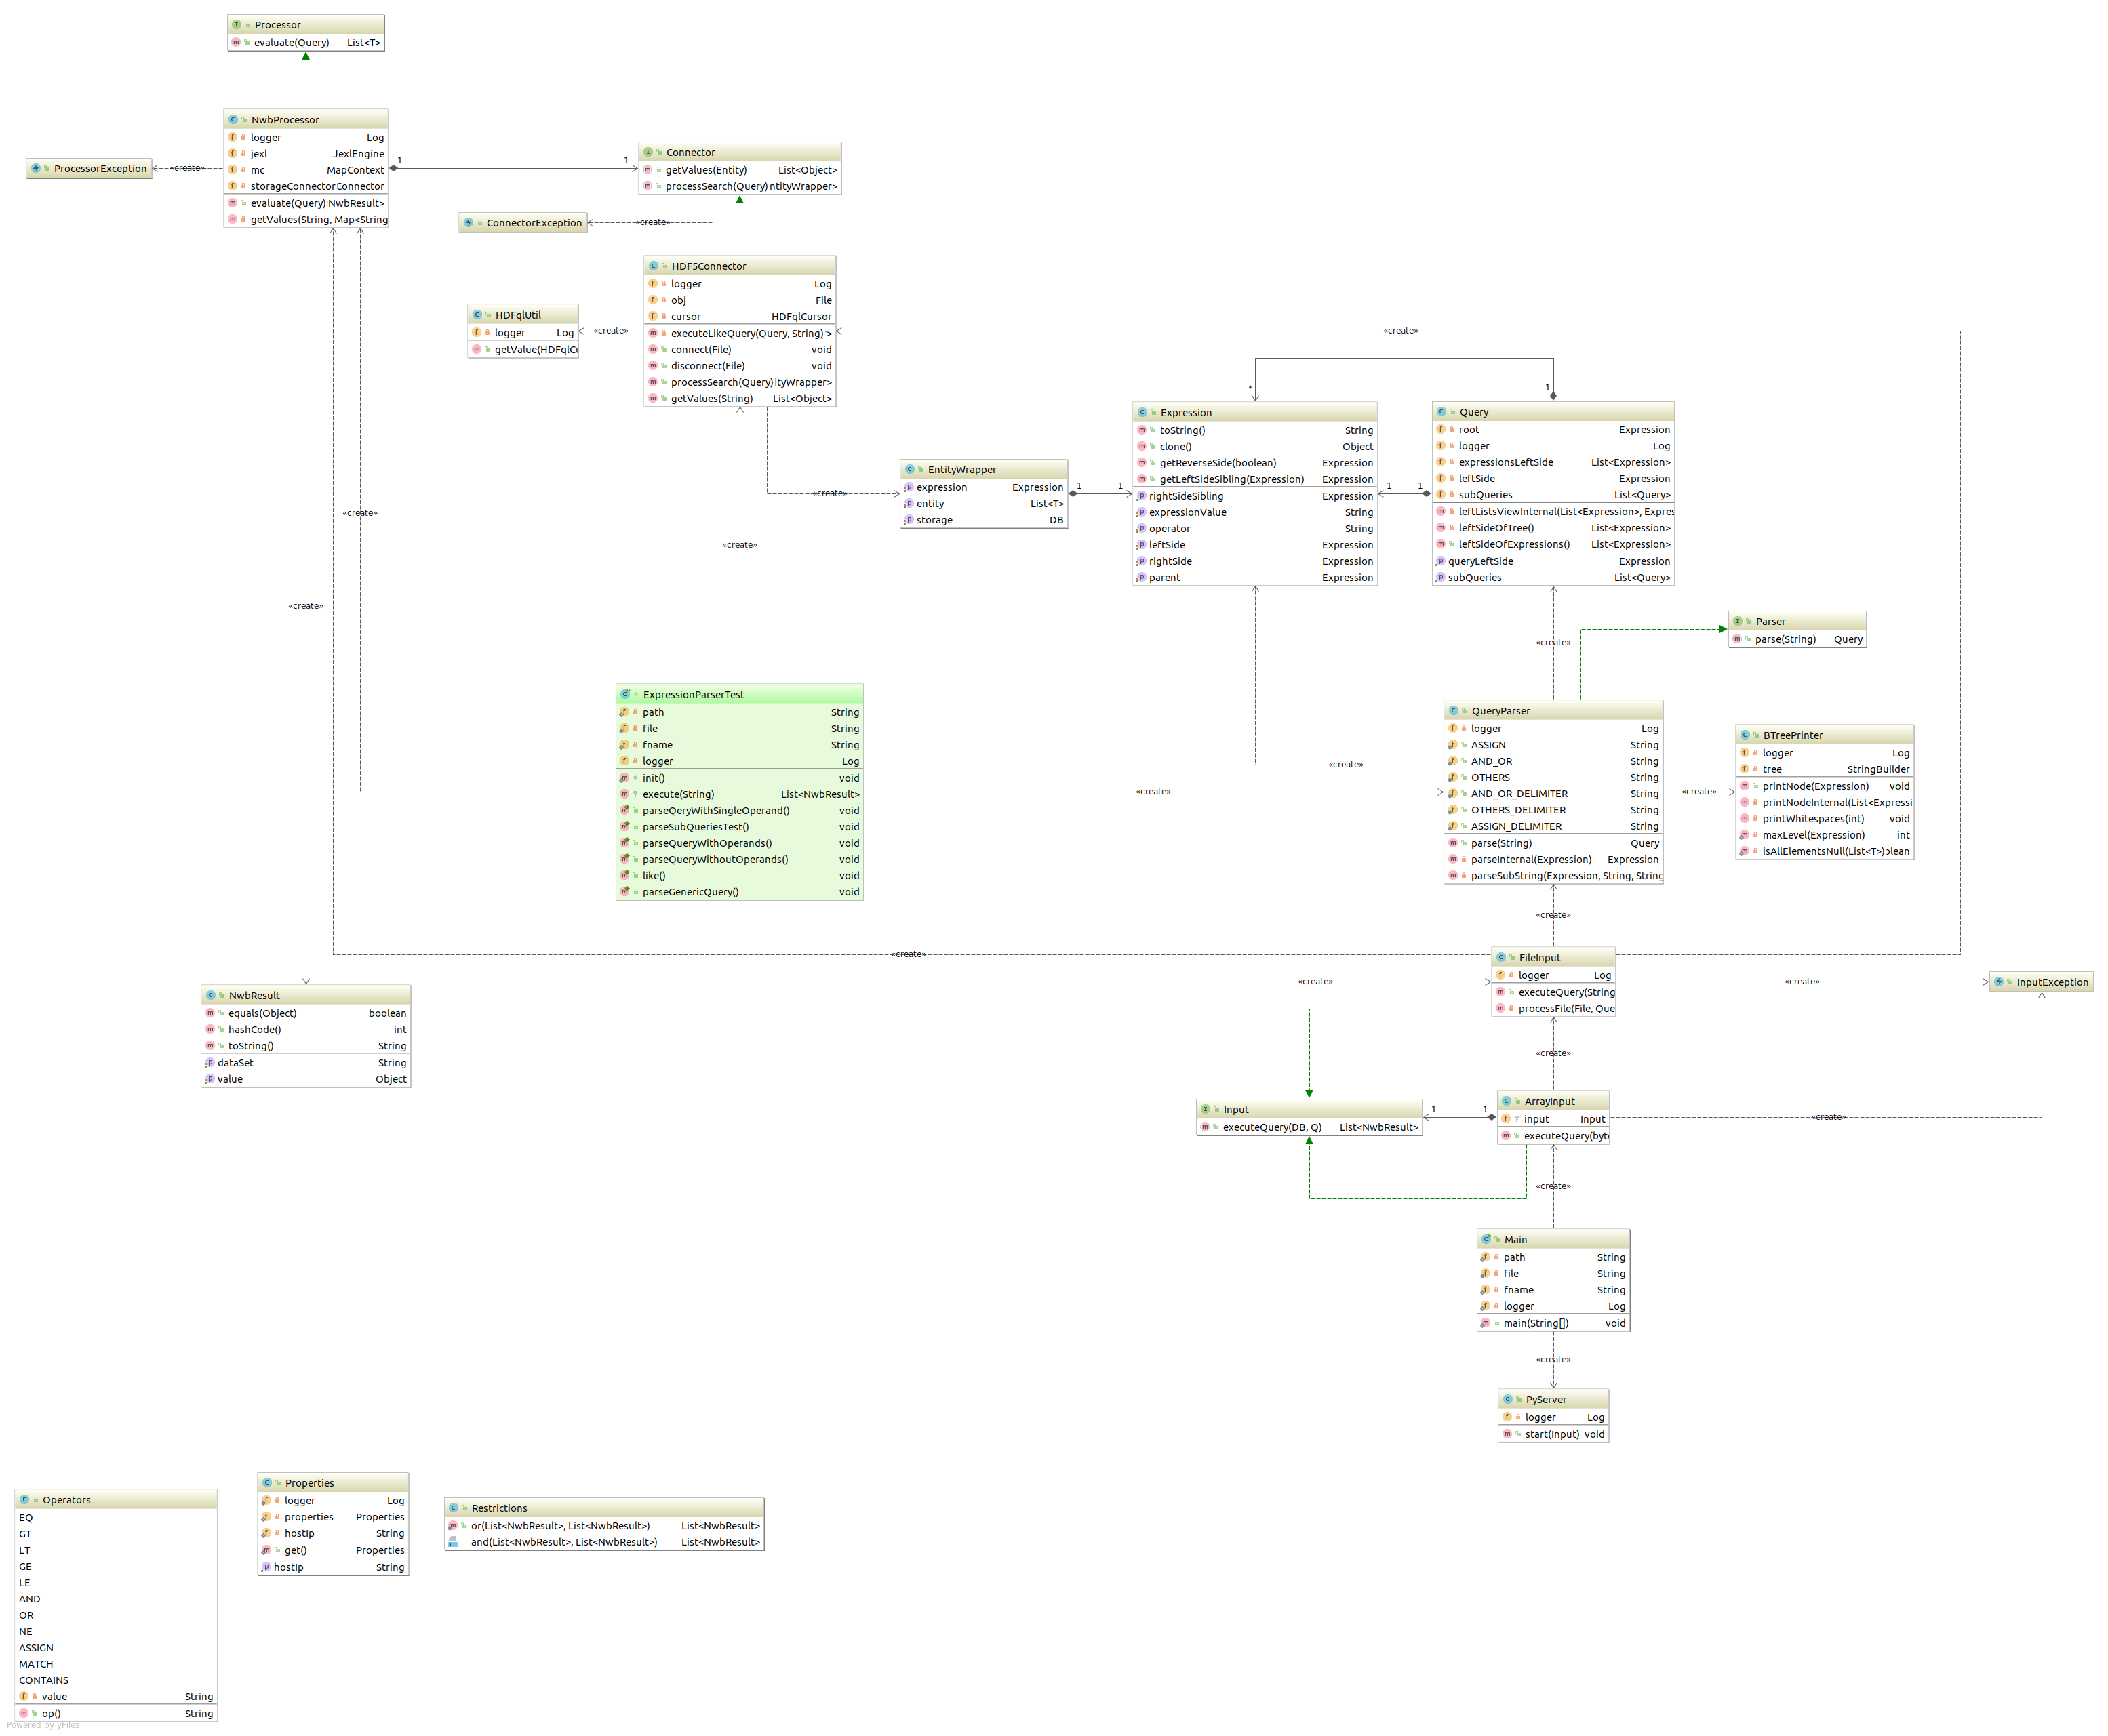
\includegraphics[width=18cm]{diagram}
% figure caption is below the figure
\caption[UML Diagram of the NWB Query Engine.]{\textbf{UML Diagram of the NWB Query Engine.} A standard UML class diagram notation is used. Classes are marked by "C" letter in a blue circle. Interfaces are marked by "I" letter in a green circle. Solid lines with open arrowhead represent association. Dashed lines with unfilled arrowhead represent inheritance. Filled diamonds shapes at the end of lines represent a composition relationship. Dashed lines with open arrowhead represents a dependency.}
\label{fig:diagram}
\end{figure}


\subsection{Implementation}
\label{Implementation}

From the implementation point of view the top component \emph{QueryParser} implements a grammar described in Section \ref{Query_Grammar} and returns a \emph{Query} object. The Query object is a wrapper for a list of expressions represented by an object \emph{Expression}. Such a parsed query is an input point of \emph{HDF5Connector}. The connector executes the query in a NWB file and returns results wrapped in a list of \emph{NWBResult} objects. The core of HDF5 connector uses methods from the HDFql library. Technically it is a  C++ solution integrated with a Java application by a provided wrapper. Evaluation of queries is ensured by \emph{NWBProcessor}. The modules communicates via interfaces. Namely \emph{Connector} is an interface for \emph{HDF5Connector}, \emph{Parser} is an interface for \emph{QueryParser} and \emph{Processor} is an interface for \emph{NWBProcessor}. The input point of the application (which inputs the queries) is an  \emph{Input} interface. Their two implementations enable reading of data from a file (\emph{FileInput} class) or from a byte array (\emph{ByteArray} class) respectively. Last described class is \emph{PyServer} that enables calling the query engine from a python code as mentioned in Section \ref{Architecture}. An UML diagram showing complete implementation is in Figure \ref{fig:diagram}.

From the technological stack of view the core components are implemented in a Java language that facilitates the implementation of the sufficiently robust and abstract tool its future extensions is easy and require only minimal programming effort. 

\subsubsection{Python Gateway}
\label{Python_Gateway}

Nowadays Python is the most popular and most used language in neuroscience. There are even research topics \citep{10.3389/fninf.2015.00011} that aims to encourage interoperability and collaboration between python developers. There is described a lot of neuroscience applications based on the python language in a lot of domains included. It is e. g. a python package for graph-theoretical analysis of biomolecular networks employed it to investigation of protein networks associated with Azheimer's disease. Also lot of python based libraries for machine learning exist. E. g. PyMVPA a  framework for analysis of fMRI, EEG and MEG, DataViewer 3D is an application for displaying and integrating data from multiple neuroimaging modalities. Next, VisionEgg and PsychoPy, both are applications using OpenGL to generate temporally and spatially precise, arbitrarily complex visual stimulation protocols.  Moreover lot of tools are written on the top of existing solutions written in C/C++ or Java languages. 

Existing approaches motivate us to implement a Python Gateway that provides an easy-to-use possibility of calling the NWB Query engine without knowledge of internal implementation or used technologies. 

We used a Python-Java bridge Py4j\footnote{\url{https://www.py4j.org/}} that allows calling of Java code from a Python program. On the Query Engine side we implemented a simple Python Server what is a Py4j GatewayServer that runs and listen on a defined port. It allows execution of method defined as an entry point. The entry point in the Python Gateway is the \emph{Input} interface explained in Section \ref{Implementation}. 

When the server is running the user on the client side can execute simple code described in Listing \ref{lst:python_code}.

\begin{lstlisting}[caption={\emph{Example of calling the python server.} In the first step a \emph{JavaGateway} library is imported. Once a Java Gateway is created the user can call the \emph{executeQuery} method with two parameters: (1) input file/dir and (2) required query. Next lines iterates over the result and print individual datasets},label={lst:python_code}]
 >>> from py4j.java_gateway import JavaGateway
 >>> from py4j.java_gateway import GatewayParameters
 >>> gateway = JavaGateway() # for localhost
 >>> gateway = JavaGateway(gateway_parameters=GatewayParameters(address='remote host ip')) # or for remote host
 >>> res = gateway.executeQuery("file or dir with nwb files", "query")
 >>> for x in res:
 ...     print (x)
\end{lstlisting}

\subsection{Web interface}
\label{web_interface}

Despite the fact the NWB Query engine can be easily deployed and used there are still not experienced users for whom it could be an obstacle. One reason could be the fact that lot of laboratories do not have system administrators who could deploy such a tool to laboratory computers. Moreover current trends go toward to cloud based solutions installed on remote servers accessible via thin clients from users desktops. A concept of shifting neurodata laboratories from locally maintained systems to a cloud based solutions are discussed e. g. in \citep{ROSENTHAL2010342}. These solutions do not require to install software on individual computer but are maintained centrally on a remote servers. 

Following this trend and to to make working with the NWB Query engine even much simpler we provided a web based system that allows execution of queries comfortably from a web browser. Another motivation for us have been an assumption that data in laboratories are stored in a central data storage uploaded from individual working stations. We have supposed that such a web interface facilitates searching within data without requiring specific software installation on users computers.

The web interface preview is in Figure \ref{web_interface}. It is a simple web page with basic information about the tool. A central element is a search box for the user input query. When the user run a query the NWB query engine is called on the background. This task can be time consuming because lot of data can be stored. For that reason the web page is implemented dynamically. It means that data are read and displayed in a sequence once they are loaded. Moreover a progress bar informs the user how many data files have been browsed already. Once required files are found the user can download them.

From the technological point of view the web Interface is implemented in the Spring framework. It is an implementation of the Dependency Injection design pattern that allows developers to easily integrate individual modules to the core application. It also integrates other used technologies. Namely Wicket framework, used as a user layer. It is an Ajax-based framework used for implementation of dynamic data loading. The design of the web pages is implemented in the Apache Bootstrap framework. Its is a library of predefined CSS templates ready to be immediately deployed.


\begin{figure}
% Use the relevant command to insert your figure file.
% For example, with the graphicx package use
  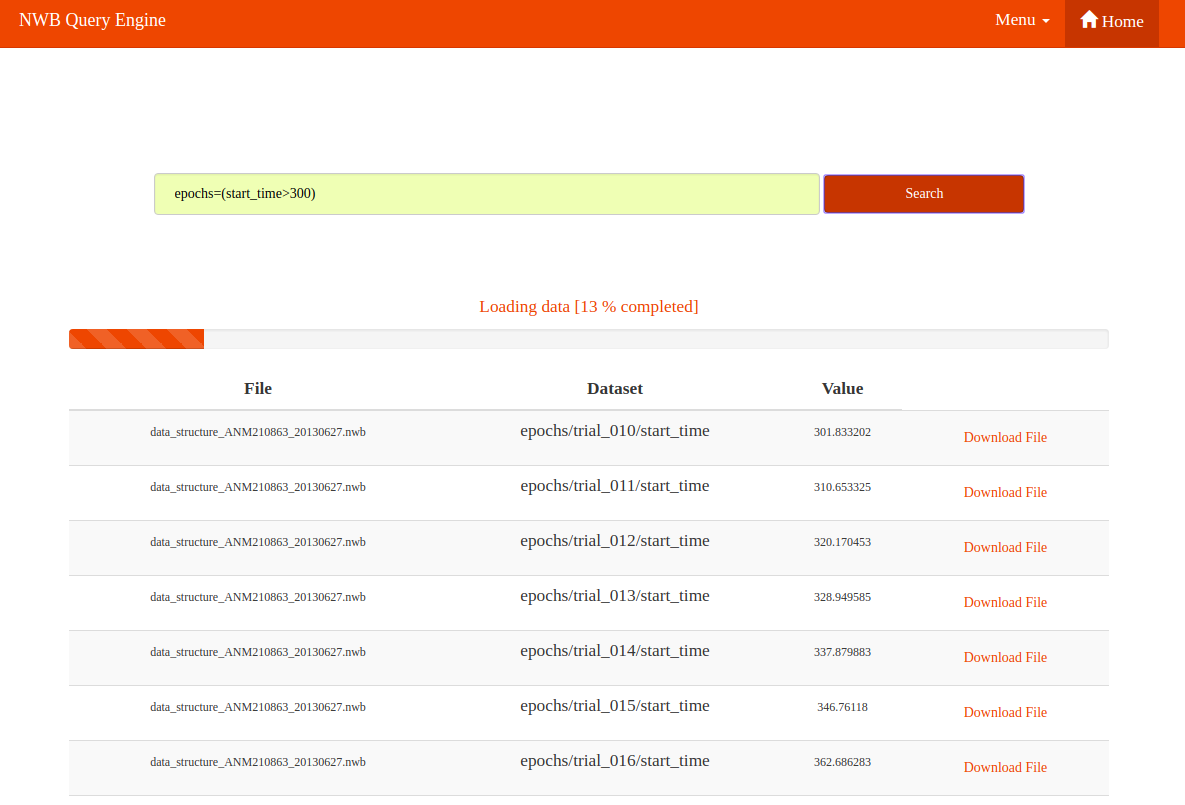
\includegraphics[width=17cm]{nwb-query-engine-web}
% figure caption is below the figure
\caption{\emph{NWB Query Engine Web Interface Preview.} The web interface provides a Google-like search box. The progress bar informs the user the percentage of browsed files. A table with result is displayed gradually. The table informs the user about a name of file with requested data, the name of dataset where data has been found, the current value of the dataset, and a link for downloading the file.}
\label{fig:web-interface}
\end{figure}

\begin{figure}
% Use the relevant command to insert your figure file.
% For example, with the graphicx package use
  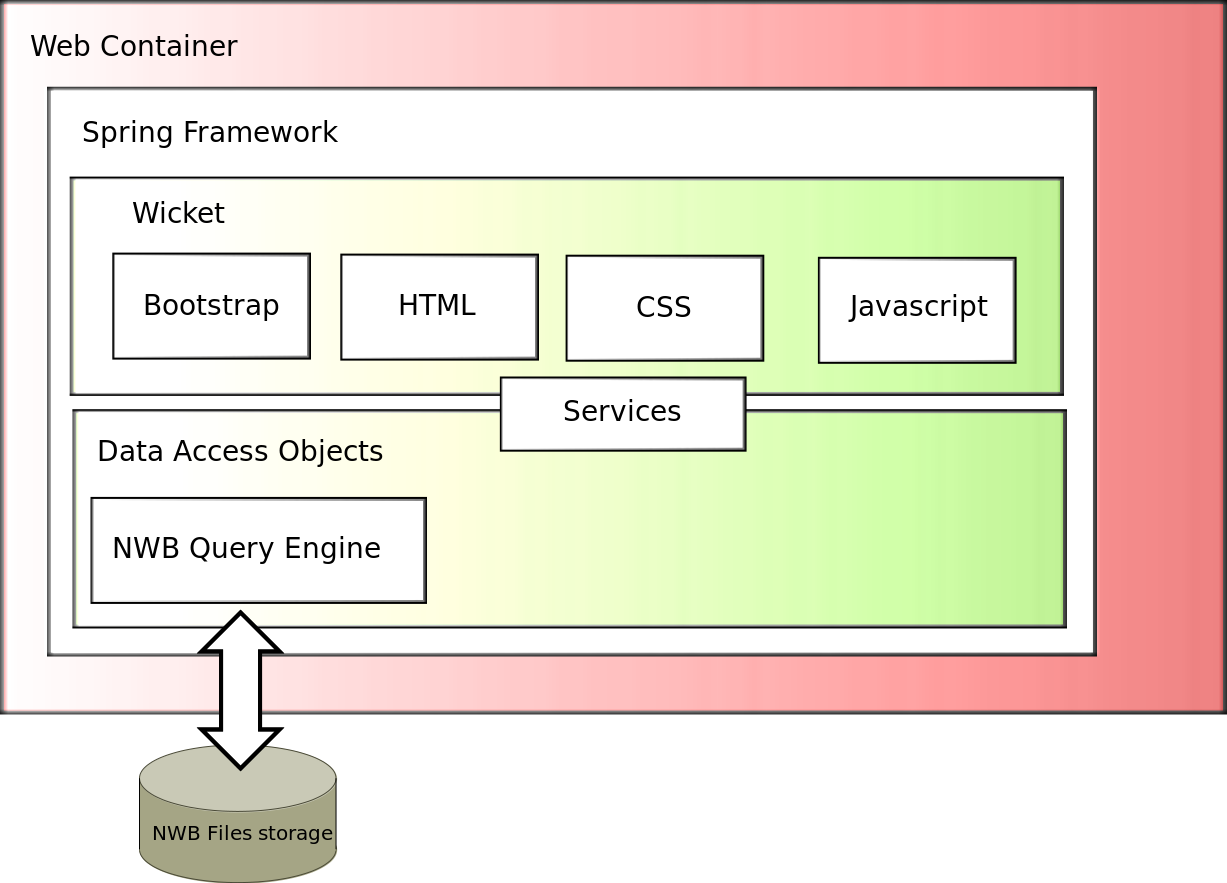
\includegraphics[width=17cm]{web-interface}
% figure caption is below the figure
\caption{\textbf{Web Interface the NWB Query Engine.} The Web Interface is implemented in a common three layer architecture. We used the Spring Framwework. The data layer accesses data via the NWB Query Engine and returns results to the view layer via the service layer. The view layer is implemented in the Wicket framework.}
\label{fig:architecture}
\end{figure}

\subsection{User Guide}

Both projects, The NWB Query Engine\footnote{\url{https://github.com/jezekp/NwbQueryEngine}} and the web interface\footnote{\url{https://github.com/jezekp/nwbQueryEngineWebInterface}} are hosted in GitHub repositories. 

The installation of both projects is step-by-step described in project repositories.  Minimal common requirement for running is to have installed JRE 8\footnote{\url{http://www.oracle.com/technetwork/java/javase/downloads/jre8-downloads-2133155.html}}. When the query engine is called from a python code a py4j python library\footnote{\url{https://www.py4j.org/install.html}} is required in python installation. The web interface runs in the Apache Tomcat\footnote{\url{https://tomcat.apache.org/download-80.cgi}} web container. Being aware of the fact that running and configuring a tomcat container could be an obstacle for some user we also provided a docker\footnote{\url{https://www.docker.com/}} file for easy build of a docker image.

The NWB Query Engine can be operated in three ways:
\begin{enumerate}
 \item A standalone application - In this case running the tool as a command line application taking two arguments is possible. The first argument is a NWB file or a directory containing NWB files while the second one is a query. The results are printed to a standard output.
 \item A library function - The Query engine is integrated to a 3rd party tool. An input point is the \emph{Input} interface as mentioned in Section \ref{Implementation}. The client program only calls methods from this interface. Results are returned in the \emph{NWBResult} object. Easy integration with third-party tools is ensured by a Maven\footnote{https://maven.apache.org/} artifact released and described in the project repository.
 \item A Python server - If the Query engine is run with a command line parameter \emph{pyserver} it starts as a Python Gateway. Now it can be called from a python code as described in Section \ref{Python_Gateway}.
\end{enumerate}


\section{Discussion}
\label{Discussion}

This paper is a part of the current approach to provide a standardized way to store and access data produced in neurophysiology. Long term experiences of interested laboratories resulted in a development of a unified data format, Neurodata Without Borders. Taking into account the fact that once data are stored they must be effectively queried an innovative approach and its technological design is presented. Because of innovativeness of the NWB format a new solution implemented basically from scratch has been an inevitable step. However described use-cases provided a good overview of requirements according them the presented solution has been implemented.

Even though the current implementation is specific to the NWB data format the system is based on general concepts that can be reused in other domains. Moreover implemented modular structure facilitates its extension to various data sources.

As a starting point we took into account defined structure of the NWB data format. The typical neurophysiology experimental set-ups gave us a specification of the developed query engine. 

We also tested solutions working on top of relational databases such as DataJoint. Although the NWB data format is based on a different concept then relational database based solutions we tool an inspiration of relational algebra implemented in DataJoint. We also took into account a need to maintain a support for python programmers. 

Because the NWB data format is implemented in HDF5 we took into account also the internal structure of this data container. Based on the use-cases and the NWB format structure we found that most flexible solution would require searching on the granularity given by the system of groups, datasets and attributes.

Based on the requirements of an easier language then SQL and on the known structure of the format, and relational algebra described in DataJoint we implemented a simple query language containing basic relational operations executed on groups, datasets or attributes.

The query language we presented is simple to use because it does not require any specific knowledge of database systems. It uses simple arithmetical and logical operators. Unstructured textural data can be browsed by a LIKE operator allowing to get a complete text according to a substring. 

The main advantage of SQL is its optimization in database systems. Data are indexed and queries are optimized within a database engine so querying of such data is fast. In this work such indexation and optimization has not been possible because the query engine does not know internal implementation of a concrete data storage. Once data are annotated by some sophisticated techniques based on controlled vocabularies or semantic web languages the presented query language could operate on the top of such annotated data and provide faster searching mechanism.

A generic and easy-to-use application practically implementing the presented query language is also presented. This application contains several modules easily extensible by implementing of connectors for various data storages. We present here an implementation of HDF5 connector that allows running of queries on the NWB files implemented in HDF5. However if in the future a different data storage is required the query language can be easily extended by implementing another connector. Connectors communicate with the core engine by an interface. That ways users to implement they own connector for a different data storages without affecting rest of the system. Such connectors could include e. g. a connector for the NIX data format, matlab data formats or eventually a connector serving as a bridge to SQL.


The HDF5 connector internally uses the HDFql library that facilitates accessing of groups and datasets in an HDF5 file. All other executions are performed on the top of this connector. It in result makes the query engine independent of the HDF5 implementation. The usage of HDFql could be possibly a limiting factor if the support of this library ended. However due to  separation of the modules would not affect the engine core. 

For python users we provided a python gateway. Non programmers can use a web based interface that can be easily installed on a laboratory server and accessed by a complete team participating in experiments.

There are two versions of the NWB format. We have fully tested the presented solution on the NWB version 1.0 on a set of more then one hundred single data files. On the version 2.0 we are limited only by the current non-existence of files stored in this version. However the presented concepts are defined and implemented sufficiently general to work on the new version and also on possible future versions.

The current data files are usually stored on laboratory computers not shared via the Internet. Or there are data that are provided via custom web services or web portals. Such approach prevents downloading data by a unified way. There are proposed solution e. g. INCF Dataspace\footnote{https://github.com/INCF/ids-tools/wiki/Using-the-INCF-Dataspace} that aim is to provide a federated data network accessible via the iRods platform \citep{rajasekar2010irods}. Data within this network are then accessed as if they were in a single file system. 

The NWB Query engine is supposed to be installed on a single file system as well. If data were federated in a distributed network the NWB Query engine could be installed in this network as well. Such an approach would enable easy searching of data withing this network. Because the presented web interface runs on the top of the NWB query engine the data could be easily browsed by a unified web interface over all this network.

\todo[inline]{Add aggregation fuctions such as count, max, min, etc as a future work?)}


\section*{Conflict of Interest Statement}
%All financial, commercial or other relationships that might be perceived by the academic community as representing a potential conflict of interest must be disclosed. If no such relationship exists, authors will be asked to confirm the following statement: 

The authors declare that the research was conducted in the absence of any commercial or financial relationships that could be construed as a potential conflict of interest.

\section*{Author Contributions}

The Author Contributions section is mandatory for all articles, including articles by sole authors. If an appropriate statement is not provided on submission, a standard one will be inserted during the production process. The Author Contributions statement must describe the contributions of individual authors referred to by their initials and, in doing so, all authors agree to be accountable for the content of the work. Please see  \href{http://home.frontiersin.org/about/author-guidelines#AuthorandContributors}{here} for full authorship criteria.

\section*{Funding}
Details of all funding sources should be provided, including grant numbers if applicable. Please ensure to add all necessary funding information, as after publication this is no longer possible.

\section*{Acknowledgments}
This is a short text to acknowledge the contributions of specific colleagues, institutions, or agencies that aided the efforts of the authors.

\section*{Supplemental Data}
 \href{http://home.frontiersin.org/about/author-guidelines#SupplementaryMaterial}{Supplementary Material} should be uploaded separately on submission, if there are Supplementary Figures, please include the caption in the same file as the figure. LaTeX Supplementary Material templates can be found in the Frontiers LaTeX folder 


\bibliographystyle{frontiersinSCNS_ENG_HUMS} % for Science, Engineering and Humanities and Social Sciences articles, for Humanities and Social Sciences articles please include page numbers in the in-text citations
%\bibliographystyle{frontiersinHLTH&FPHY} % for Health, Physics and Mathematics articles
\bibliography{nwb-query-engine}

%%% Make sure to upload the bib file along with the tex file and PDF
%%% Please see the test.bib file for some examples of references


\end{document}
